% Template for PLoS
% Version 3.5 March 2018
%
% % % % % % % % % % % % % % % % % % % % % %
%
% -- IMPORTANT NOTE
%
% This template contains comments intended 
% to minimize problems and delays during our production 
% process. Please follow the template instructions
% whenever possible.
%
% % % % % % % % % % % % % % % % % % % % % % % 
%
% Once your paper is accepted for publication, 
% PLEASE REMOVE ALL TRACKED CHANGES in this file 
% and leave only the final text of your manuscript. 
% PLOS recommends the use of latexdiff to track changes during review, as this will help to maintain a clean tex file.
% Visit https://www.ctan.org/pkg/latexdiff?lang=en for info or contact us at latex@plos.org.
%
%
% There are no restrictions on package use within the LaTeX files except that 
% no packages listed in the template may be deleted.
%
% Please do not include colors or graphics in the text.
%
% The manuscript LaTeX source should be contained within a single file (do not use \input, \externaldocument, or similar commands).
%
% % % % % % % % % % % % % % % % % % % % % % %
%
% -- FIGURES AND TABLES
%
% Please include tables/figure captions directly after the paragraph where they are first cited in the text.
%
% DO NOT INCLUDE GRAPHICS IN YOUR MANUSCRIPT
% - Figures should be uploaded separately from your manuscript file. 
% - Figures generated using LaTeX should be extracted and removed from the PDF before submission. 
% - Figures containing multiple panels/subfigures must be combined into one image file before submission.
% For figure citations, please use "Fig" instead of "Figure".
% See http://journals.plos.org/plosone/s/figures for PLOS figure guidelines.
%
% Tables should be cell-based and may not contain:
% - spacing/line breaks within cells to alter layout or alignment
% - do not nest tabular environments (no tabular environments within tabular environments)
% - no graphics or colored text (cell background color/shading OK)
% See http://journals.plos.org/plosone/s/tables for table guidelines.
%
% For tables that exceed the width of the text column, use the adjustwidth environment as illustrated in the example table in text below.
%
% % % % % % % % % % % % % % % % % % % % % % % %
%
% -- EQUATIONS, MATH SYMBOLS, SUBSCRIPTS, AND SUPERSCRIPTS
%
% IMPORTANT
% Below are a few tips to help format your equations and other special characters according to our specifications. For more tips to help reduce the possibility of formatting errors during conversion, please see our LaTeX guidelines at http://journals.plos.org/plosone/s/latex
%
% For inline equations, please be sure to include all portions of an equation in the math environment.  For example, x$^2$ is incorrect; this should be formatted as $x^2$ (or $\mathrm{x}^2$ if the romanized font is desired).
%
% Do not include text that is not math in the math environment. For example, CO2 should be written as CO\textsubscript{2} instead of CO$_2$.
%
% Please add line breaks to long display equations when possible in order to fit size of the column. 
%
% For inline equations, please do not include punctuation (commas, etc) within the math environment unless this is part of the equation.
%
% When adding superscript or subscripts outside of brackets/braces, please group using {}.  For example, change "[U(D,E,\gamma)]^2" to "{[U(D,E,\gamma)]}^2". 
%
% Do not use \cal for caligraphic font.  Instead, use \mathcal{}
%
% % % % % % % % % % % % % % % % % % % % % % % % 
%
% Please contact latex@plos.org with any questions.
%
% % % % % % % % % % % % % % % % % % % % % % % %

\documentclass[10pt,letterpaper]{article}
\usepackage[top=0.85in,left=2.75in,footskip=0.75in]{geometry}

% amsmath and amssymb packages, useful for mathematical formulas and symbols
\usepackage{amsmath,amssymb}

% Use adjustwidth environment to exceed column width (see example table in text)
\usepackage{changepage}

% Use Unicode characters when possible
\usepackage[utf8x]{inputenc}

% textcomp package and marvosym package for additional characters
\usepackage{textcomp,marvosym}

% cite package, to clean up citations in the main text. Do not remove.
\usepackage{cite}

% Use nameref to cite supporting information files (see Supporting Information section for more info)
\usepackage{nameref,hyperref}

% line numbers
\usepackage[right]{lineno}

% ligatures disabled
\usepackage{microtype}
\DisableLigatures[f]{encoding = *, family = * }

% color can be used to apply background shading to table cells only
\usepackage[table]{xcolor}

% array package and thick rules for tables
\usepackage{array}

% create "+" rule type for thick vertical lines
\newcolumntype{+}{!{\vrule width 2pt}}

% create \thickcline for thick horizontal lines of variable length
\newlength\savedwidth
\newcommand\thickcline[1]{%
  \noalign{\global\savedwidth\arrayrulewidth\global\arrayrulewidth 2pt}%
  \cline{#1}%
  \noalign{\vskip\arrayrulewidth}%
  \noalign{\global\arrayrulewidth\savedwidth}%
}

% \thickhline command for thick horizontal lines that span the table
\newcommand\thickhline{\noalign{\global\savedwidth\arrayrulewidth\global\arrayrulewidth 2pt}%
\hline
\noalign{\global\arrayrulewidth\savedwidth}}


% Remove comment for double spacing
%\usepackage{setspace} 
%\doublespacing

% Text layout
\raggedright
\setlength{\parindent}{0.5cm}
\textwidth 5.25in 
\textheight 8.75in

% Bold the 'Figure #' in the caption and separate it from the title/caption with a period
% Captions will be left justified
\usepackage[aboveskip=1pt,labelfont=bf,labelsep=period,justification=raggedright,singlelinecheck=off]{caption}
\renewcommand{\figurename}{Fig}

% Use the PLoS provided BiBTeX style
\bibliographystyle{plos2015}

% Remove brackets from numbering in List of References
\makeatletter
\renewcommand{\@biblabel}[1]{\quad#1.}
\makeatother



% Header and Footer with logo
\usepackage{lastpage,fancyhdr,graphicx}
\usepackage{epstopdf}
%\pagestyle{myheadings}
\pagestyle{fancy}
\fancyhf{}
%\setlength{\headheight}{27.023pt}
%\lhead{\includegraphics[width=2.0in]{PLOS-submission.eps}}
\rfoot{\thepage/\pageref{LastPage}}
\renewcommand{\headrulewidth}{0pt}
\renewcommand{\footrule}{\hrule height 2pt \vspace{2mm}}
\fancyheadoffset[L]{2.25in}
\fancyfootoffset[L]{2.25in}
\lfoot{\today}

%% Include all macros below

\newcommand{\lorem}{{\bf LOREM}}
\newcommand{\ipsum}{{\bf IPSUM}}

%% END MACROS SECTION


\begin{document}
\vspace*{0.2in}

% Title must be 250 characters or less.
\begin{flushleft}
{\Large
\textbf\newline{Nested stochastic block models applied to the analysis of single cell data} % Please use "sentence case" for title and headings (capitalize only the first word in a title (or heading), the first word in a subtitle (or subheading), and any proper nouns).
}
\newline
% Insert author names, affiliations and corresponding author email (do not include titles, positions, or degrees).
\\
Leonardo Morelli\textsuperscript{1,2},
Valentina Giansanti\textsuperscript{1, 3},
Davide Cittaro\textsuperscript{1*},
\\
\bigskip
\textbf{1} Center for Omics Sciences, IRCCS San Raffaele Institute, Milan, Italy
\\
\textbf{2} Universit\`{a} Vita-Salute San Raffaele, Milan, Italy
\\
\textbf{3} Department of Informatics, Systems and Communication, University of Milano-Bicocca, Milan, Italy
\\
\bigskip

% Insert additional author notes using the symbols described below. Insert symbol callouts after author names as necessary.
% 
% Remove or comment out the author notes below if they aren't used.
%
% Primary Equal Contribution Note
%\Yinyang These authors contributed equally to this work.

% Additional Equal Contribution Note
% Also use this double-dagger symbol for special authorship notes, such as senior authorship.
%\ddag These authors also contributed equally to this work.

% Current address notes
%\textcurrency Current Address: Dept/Program/Center, Institution Name, City, State, Country % change symbol to "\textcurrency a" if more than one current address note
% \textcurrency b Insert second current address 
% \textcurrency c Insert third current address

% Deceased author note
%\dag Deceased

% Group/Consortium Author Note
%\textpilcrow Membership list can be found in the Acknowledgments section.

% Use the asterisk to denote corresponding authorship and provide email address in note below.
* cittaro.davide@hsr.it

\end{flushleft}
% Please keep the abstract below 300 words
\section*{Abstract}
Single cell profiling has been proven to be a powerful tool in molecular biology to understand the complex behaviours of heterogeneous system. While properties of single cells is the primary endpoint of such analysis, these are typically clustered to underpin the common determinants that can be used to describe functional properties of the cell mixture under investigation. Several approaches have been proposed to identify cell clusters; while this is matter of active research, one popular approach is based on community detection in neighbourhood graphs by optimisation of modularity. In this paper we propose an alternative solution to this problem, based on nested Stochastic Block Models; we show a threefold advantage of our approach as it is able to correctly identify cell groups, it returns a meaningful hierarchical structure and, lastly, it provides a statistical measure of association between cells and the assigned clusters.


% Please keep the Author Summary between 150 and 200 words
% Use first person. PLOS ONE authors please skip this step. 
% Author Summary not valid for PLOS ONE submissions.   
\section*{Author summary}
Identification of cell types is a key step of many single cell experiments. Many of the approaches to achieve this goal converge on the analysis of the graph representing cell-wise similarity by optimisation of modularity. While fast, this method does not provide a robust estimation of the number of groups, and it leaves large room of arbitrariness in the choice of appropriate resolution. To overcome these limitations, we propose a strategy based on nested stochastic block models. We show our method is accurate and provides a rich description of cell groups and their relationships.

\linenumbers

% Use "Eq" instead of "Equation" for equation citations.
\section*{Introduction}
Transcriptome analysis at single cell level by RNA sequencing (scRNA-seq) is a technology growing in popularity and applications \cite{svensson_2018}. It has been applied to study the biology of complex tissues \cite{guo_2018, ventotormo_2018}, tumor dynamics \cite{rozenblattrosen_2020, tirosh_2016, patel_2014, neftel_2019}, development \cite{rosenberg_2018, wagner_2018} and to describe whole organisms \cite{plass_2018, regev_2017}.

A key step in the analysis of scRNA-seq data and, more in general, of single cell data, is the identification of cell populations, groups of cells sharing similar properties. Several approaches have been proposed to achieve this task, based on well established clustering techniques \cite{wang_2017, lin_2017}, consensus clustering \cite{huh_2020, kiselev_2017} and deep learning \cite{li_2020}; many more have been recently reviewed \cite{krzak_2019, kiselev_2019} and benchmarked \cite{du_2018}. As the popularity of single cell analysis frameworks Seurat \cite{butler_2018} and Scanpy \cite{wolf_2018} raised, methods based instead on graph partitioning became the \emph{de facto} standards. Such methods require the construction of a cell neighbourhood graph (\emph{e.g.} by \emph{k }Nearest Neighbours, \emph{k}NN) which is then partitioned into communities; the latter step is typically performed using the Louvain method \cite{blondel_2008}, a fast algorithm for optimisation of graph modularity. While fast, this method does not guarantee that small communities in large networks are well defined. To overcome its limits, a more recent approach, the Leiden algorithm \cite{traag_2019}, has been implemented and it has been quickly adopted in the analysis of single cell data, for example by Scanpy and PhenoGraph \cite{levine_2015}. In addition to Newman's modularity \cite{newman_2004}, other definitions currently used in single cell analysis make use of a resolution parameter \cite{traag_2011, reichardt_2006} . In lay terms, resolution works as a threshold on the density within communities: lowering the resolution results in less and sparser communities and \emph{viceversa}. Identification of an appropriate resolution has been recognised as a major issue \cite{lhnemann_2020}, also because it requires the definition of a mathematical property (clusters) over biological entities (the cell groups), with little formal description of the latter. In addition, the larger the dataset, the harder is to identify small cell groups, as a consequence of the well-known resolution limit \cite{fortunato_2007}. Moreover, it has been demonstrated that random networks can have modularity \cite{guimer_2004} and its optimisation is incapable of separating actual structure from those arising simply of statistical fluctuations of the null model. Additional solutions to cell group identification from neighbourhood graphs have been proposed, introducing resampling techniques \cite{baran_2019} or clique analysis \cite{xu_2015}. Lastly, it has been proposed that high resolution clustering, \emph{e.g.} obtained with Leiden or Louvain methods, can be refined in agglomerative way using machine learning techniques \cite{miao_2020}.

An alternative solution to community detection is the Stochastic Block Model, a generative model for graphs organized into communities \cite{holland_1983}. In this scenario, identification of cell groups requires the estimation of the proper parameters underlying the observed neighbourhood graph. According to the microcanonical formulation \cite{peixoto_2017}, the parameters are node partitions into groups and the matrix of edge counts between groups themselves. Under this model, nodes belonging to the same group have the same probability to be connected with other nodes. It is possible to include node degree among the model parameters \cite{karrer_2011}, to account for heterogeneity of degree distribution of real-world graphs. A Bayesian approach to infer parameters has been developed \cite{peixoto_2013} and implemented in the \emph{graph-tool} python library (\href{https://graph-tool.skewed.de}{https:/\slash graph-tool.skewed.de}). There, a generative model of network $\boldsymbol A$ has a probability $P(\boldsymbol A|\boldsymbol\theta, \boldsymbol b)$ where \textbf{$\boldsymbol\theta$} is the set of parameters and \textbf{\emph{$\boldsymbol b$}} is the set of partitions. The likelihood of the network being generated by a given partition can be measured by the posterior probability


%\begin{MPEquation}[!ht]
\begin{equation}
P(\boldsymbol b | \boldsymbol A) = \frac{P(\boldsymbol A|\boldsymbol\theta, \boldsymbol b)P(\boldsymbol\theta, \boldsymbol b)}{P(\boldsymbol A)}
\end{equation}
\label{MPEquationElement:820CB015-E51E-4C5A-BD9C-70E667B8F73B}
%\end{MPEquation}
and inference is performed by maximising the posterior probability. The numerator in this equation can be rewritten exponentiating the description length


%\begin{MPEquation}[!ht]
\begin{equation}
\Sigma = -\ln P(\boldsymbol A|\boldsymbol\theta, \boldsymbol b) - \ln P(\boldsymbol\theta, \boldsymbol b)
\end{equation}
\label{MPEquationElement:676396C0-2D6F-4084-89B1-951DE3032087}
%\end{MPEquation}
so that inference is performed by minimizing the information required to describe the data (Occam's razor); \emph{graph-tool} is able to efficiently do this by a Markov Chain Monte Carlo approach \cite{peixoto_2014}. SBM itself may fail to identify small groups in large graphs, hence hierarchical formulation has been proposed \cite{peixoto_2014_h}. Under this model, communities are agglomerated at a higher level in a block multigraph, also modelled using SBM. This process is repeated recursively until a graph with a single block is reached, creating a Nested Stochastic Block Model (nSBM).

In this work we propose nSBM for the analysis of single cell data, in particular scRNA-seq data. This approach identifies cell groups in a statistical robust way and, moreover, it is able to determine the likelihood of the grouping, thus allowing model selection. In addition, it is possible to measure the confidence of assignment to groups. We show that such information may be exploited to perfect the notion of cell groups and the identification of markers.

We developed \emph{schist} (\href{https://github.com/dawe/schist}{https:/\slash github.com\slash dawe\slash schist}), a python library compatible with \emph{scanpy}, to facilitate the adoption of nested stochastic block models in single-cell analysis.


\section*{Materials and methods}
%\subsection*{Analysis of Random data}
%Data were retrieved in \emph{scanpy} environment using \emph{sc.datasets.pbmc3k\_processed()} function. The random \emph{k}NN graph was obtained shuffling the node labels of each edge. nSBM was performed with 3 initialisations using merge-split MCMC approach. UMAP embedding was recomputed after randomisation using the shuffled graph.


\subsection*{Analysis of cell mixtures}

Data and metadata for five cell mixture profiled by Chromium 10x were downloaded from the sc-mixology repository (\href{https://github.com/LuyiTian/sc_mixology}{https:/\slash github.com\slash LuyiTian\slash sc\_mixology}). Data were analysed using scanpy v1.4.6 \cite{wolf_2018}. Cells with less than 200 genes were excluded, as genes detected in less than 3 cells. Cells with less than 5\% of mitochondrial genes were retained for subsequent analysis. Data were normalised and log-transformed; number of genes and percentage of mitochondrial genes were regressed out. nSBM was initialised three times. Analysis was performed at level 2 of the nSBM hierarchy.
Random Poisson noise was generated at given $\lambda$ (range: 0 - 1000) and added to the initial count matrix. Analysis was performed at level 2 of the nSBM hierarchy.

\subsection*{Analysis of hematopoietic differentiation}

Data were retrieved using scanpy's built-in functions and were processed as in \cite{wolf_2019}, except for \emph{k}NN graph built using 30 principal components, 30 neighbours and diffmap as embedding. Gene signatures were calculated using the following gene lists
\begin{itemize}
\item Erythroids: Gata1, Klf1, Epor, Gypa, Hba-a2, Hba-a1, Spi1
\item Neutrophils, Elane, Cebpe, Ctsg, Mpo, Gfi1
\item Monocytes, Irf8, Csf1r, Ctsg, Mpo
\end{itemize}

nSBM was completed with 3 initialisations

\subsection*{Analysis of cluster consistency}

Count matrices were downloaded from GEO using the following accession numbers: GSE133535 (Chromium 10Xv3), GSE133543 (Quartz-seq2), GSE133542 (MARS-seq) and GSE133541 (iCELL8). Data were processed according to the methods in the original paper \cite{mereu_2020}. Briefly, cells with less than 10,000 total number of reads as well as the cells having less than 65\% of the reads mapped to their reference genome were discarded. Cells in the 95th percentile of the number of genes/cell and those having less than 25\% mitochondrial gene content were included in the downstream analyses. Genes that were expressed in less than five cells were removed. Data were normalized and log-transformed, highly variable genes were detected at minimal dispersion equal to 0.5. Neighbourhood graph was built using 30 principal components and 20 neighbours. nSBM was completed with 3 initialisations. 

% Results and Discussion can be combined.
\subsection*{Overview of \emph{schist}}

\emph{schist} is a convenient wrapper to the \emph{graph-tool} python library, written in python and designed to be used with \emph{scanpy}. The most prominent function is \emph{schist.inference.nested\_model()} which takes a \emph{AnnData} object as input and fits a nested stochastic block model on the \emph{k}NN graph built with \emph{scanpy} functions (\emph{e.g.\ scanpy.tools.neighbors()}). When launched with default parameters, \emph{schist} fits a model which maximises the posterior probability of having a set of cell groups (or blocks) given a graph. \emph{schist} annotates cells in the data object with all the groups found at each level of a hierarchy. As there could be more model fits with similar entropy, \emph{schist} could explore the space of solutions with a Markov Chain Monte Carlo (MCMC) algorithm, to perform model averaging; this step is performed until it converges, that is the difference in model entropy in \emph{n} continuous iterations remains under a specified threshold. Sampling from the posterior distribution can be used to study the distribution of the number of groups, at each level. This information (group marginals) could be studied to identify the most probable number of cell groups.
Once \emph{schist} has fitted a model, it evaluates the difference in entropy given by assigning every cell to every possible group. This step generates the matrix of \emph{cell affinity}, that is the probability for a cell to belong to a specific group. A cell affinity matrix is generated and returned for every hierarchy level. We show that this information can be useful to evaluate cluster consistence.

%As the core object of \emph{graph-tool }used by \emph{schist}, the \emph{NestedBlockState}, cannot be serialised by \emph{scanpy}'s IO infrastructure, we implemented simple read\slash write functions to dump \emph{AnnData} is h5ad format, together with the \emph{NestedBlockState} as a separate file using python's \emph{pickle} library.

%\subsection*{nSBM does not return artificial cell groupings}
%One of the most relevant difference between nSBM and other methods to cluster single cells is that it relies on robust statistical modelling. In this sense, the number of groups identified strictly mirrors the amount of information contained in the data. An important consequence is that absence of information can be properly handled. To show this property we performed a simple experiment on a randomised \emph{k}NN graph. To this end we collected data for 3k PBMC (available as preprocessed data in \emph{scanpy}) and shuffled the edges of the prebuilt \emph{k}NN graph, this to keep the general graph properties unchanged. We tested that the degree distribution does not change after randomisation (Kolmogorov-Smirnov $D=0.0431$, $p=0.993$). We found that the default strategy, based on maximisation of modularity, identifies 24 cell groups, whereas nSBM does not identify any cell group. 

%This experiment is a deliberate extreme case. The quality of grouping proposed by a standard approach can be disputed in many ways, and the UMAP embedding indeed reflects the absence of any information. Nevertheless, real-world data may include an unknown amount of random noise. Hence, It is important to identify cell groups that are not artefacts arising from processing and that do not reflect the information contained in the dataset. 

%\begin{figure}[!h]
%\centering
%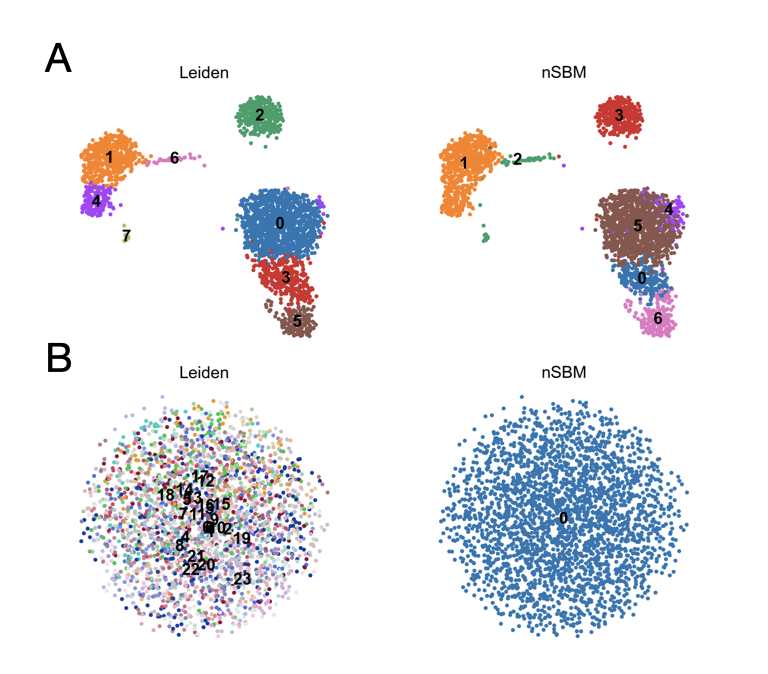
\includegraphics[keepaspectratio,width=\textwidth,height=0.4\textheight]{FIgure_Random.png}
%\caption[]{nSBM results for randomised data. (A) UMAP embedding of ~3k PBMC after standard processing with Leiden approach (left) or nSBM (right). Cell grouping is consistent for both the approaches ($ARI=0.804$). (B) UMAP embedding of the same data after randomisation of \emph{k}NN graph edges. In this case nSBM does not return any cell grouping, while optimisation of modularity finds up to 24 different cell groups}\label{FigureRandom}
%\end{figure}


\subsection*{nSBM correctly identifies cell populations}
To benchmark \emph{schist}, we tested our approach on scRNA-seq mixology data \cite{tian_2019}, in particular on a mixture of 5 cell lines profiled with Chromium 10x platform. At a first evaluation of the UMAP embedding, all lines appear well separated. Only the lung cancer line H1975 shows a certain degree of heterogeneity with some cells being embedded in other cell groups (Fig. \ref{Figure1}A). Inference on the neighbourhood graph is influenced by the graph structure itself, therefore we built multiple graphs changing the number of principal components used in PCA reduction and the number of neighbours in the \emph{k}NN graph. We then calculated the Adjusted Rand Index (\emph{ARI}) between the cell line assignments (ground truth) and the cell groups identified by nSBM at each level. We found a peak of $ARI=0.977$ with 30 principal components (PC) and 30 neighbours. In general, higher number of components and neighbours has a positive impact on the performance (Fig. \ref{Figure1}B). Conversely, if few PCs (10) or neighbors (5) are used, performances degrade, with a minimum $ARI=0.669$ at 20 PCs and 5 neighbours. If fewer PCs are used, a smaller fraction of the total variance, hence less information, is used to build the \emph{k}NN graph; if fewer neighbours are chosen, the graph is sparser and the model is fit from less edges (\nameref{S1_Fig}). Running MCMC algorithm recovers the performances of the majority of the configurations (\nameref{S2_Fig}).

Analysis of the nSBM hierarchy reveals that five levels are needed to describe the experiment (Fig. \ref{Figure1}C, upper panel), with level 2 properly catching the cell identity ($ARI = 0.977$). In addition to the five major groups, observe two small groups, summing to 11 cells, that were merged to HCC827 and H838 at hierarchy level 3. Interestingly, these groups are enriched in cells whose identity was reassigned from H1975 to H838 or HCC827 in the original paper using Demuxlet \cite{kang_2018}, indicating that nSBM was able to recognise peculiar properties and isolate them. It may be worth mention that the second best ranked group by cell affinity for these 11 cells is the correct group assigned in the original paper, except for a single cell assigned to H2228.
As a high separation between cell lines is observable, optimisation of modularity by Leiden algorithm is also able to identify cell identities with high precision, given that a proper resolution threshold is set (Fig. \ref{Figure1}C, lower panel); we found that when resolution is set to 0.05 the cell lines are properly separated ($ARI = 0.975$), with the exception of the above mentioned cells.

It is worth noting that since nSBM reflects the amount of information contained in the data, it does not return clusters when data are noisy. To demonstrate this property, we added increasing levels of random Poisson noise to the count matrix (Fig.\ref{Figure_Random}). The number of groups reported by nSBM decreases with increasing amount of noise and it is 1 (\emph{i.e.} no clusters) at $\lambda=200$, whereas a standard approach overfits data. 

These observations show that nSBM is suitable for accurate identification of cell groups, without the need of an arbitrary threshold on the resolution parameter and with the possibility to identify rare cell types in larger populations. Moreover, nSBM avoids excessive clustering of data in presence of noisy measurements.

\begin{figure}[!h]
\centering
%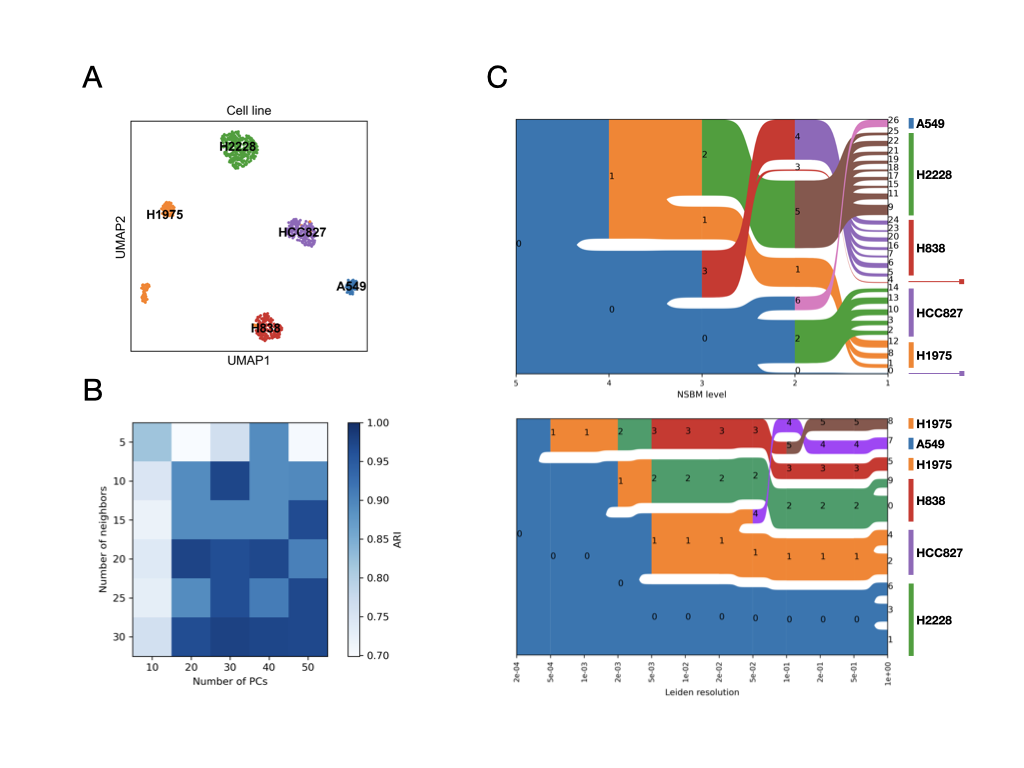
\includegraphics[keepaspectratio,width=\textwidth,height=0.6\textheight]{Figure_1.png}
\caption[]{\emph{schist} applied to scRNA-seq mixology data. (A) UMAP embedding of 10x Chromium data, cells are colored according to the given cell line in the original paper. A small number of H1975 cells are found in HCC827 and H838 clusters. (B) Heatmap showing the maximal Adjusted Rand Index for different \emph{k}NN graphs. We tested the impact of varying the number of Principal Components and the number of neighbors used in \emph{sc.pp.neighbors()} function in \emph{scanpy}. Adjusted Rand Index between the actual cell lines and the identified groups is shown. Darker blue indicates higher concordance between the model and the ground truth. (C) Alluvial plots showing the hierarchy of cell groups as identified by \emph{schist} (above) or by Leiden method at different resolution thresholds (below). The bars on the right indicate the cell identity; two marks in the \emph{schist} plot indicate two groups of cells discussed in the main text}\label{Figure1}
\end{figure}

\begin{figure}[!h]
\centering
%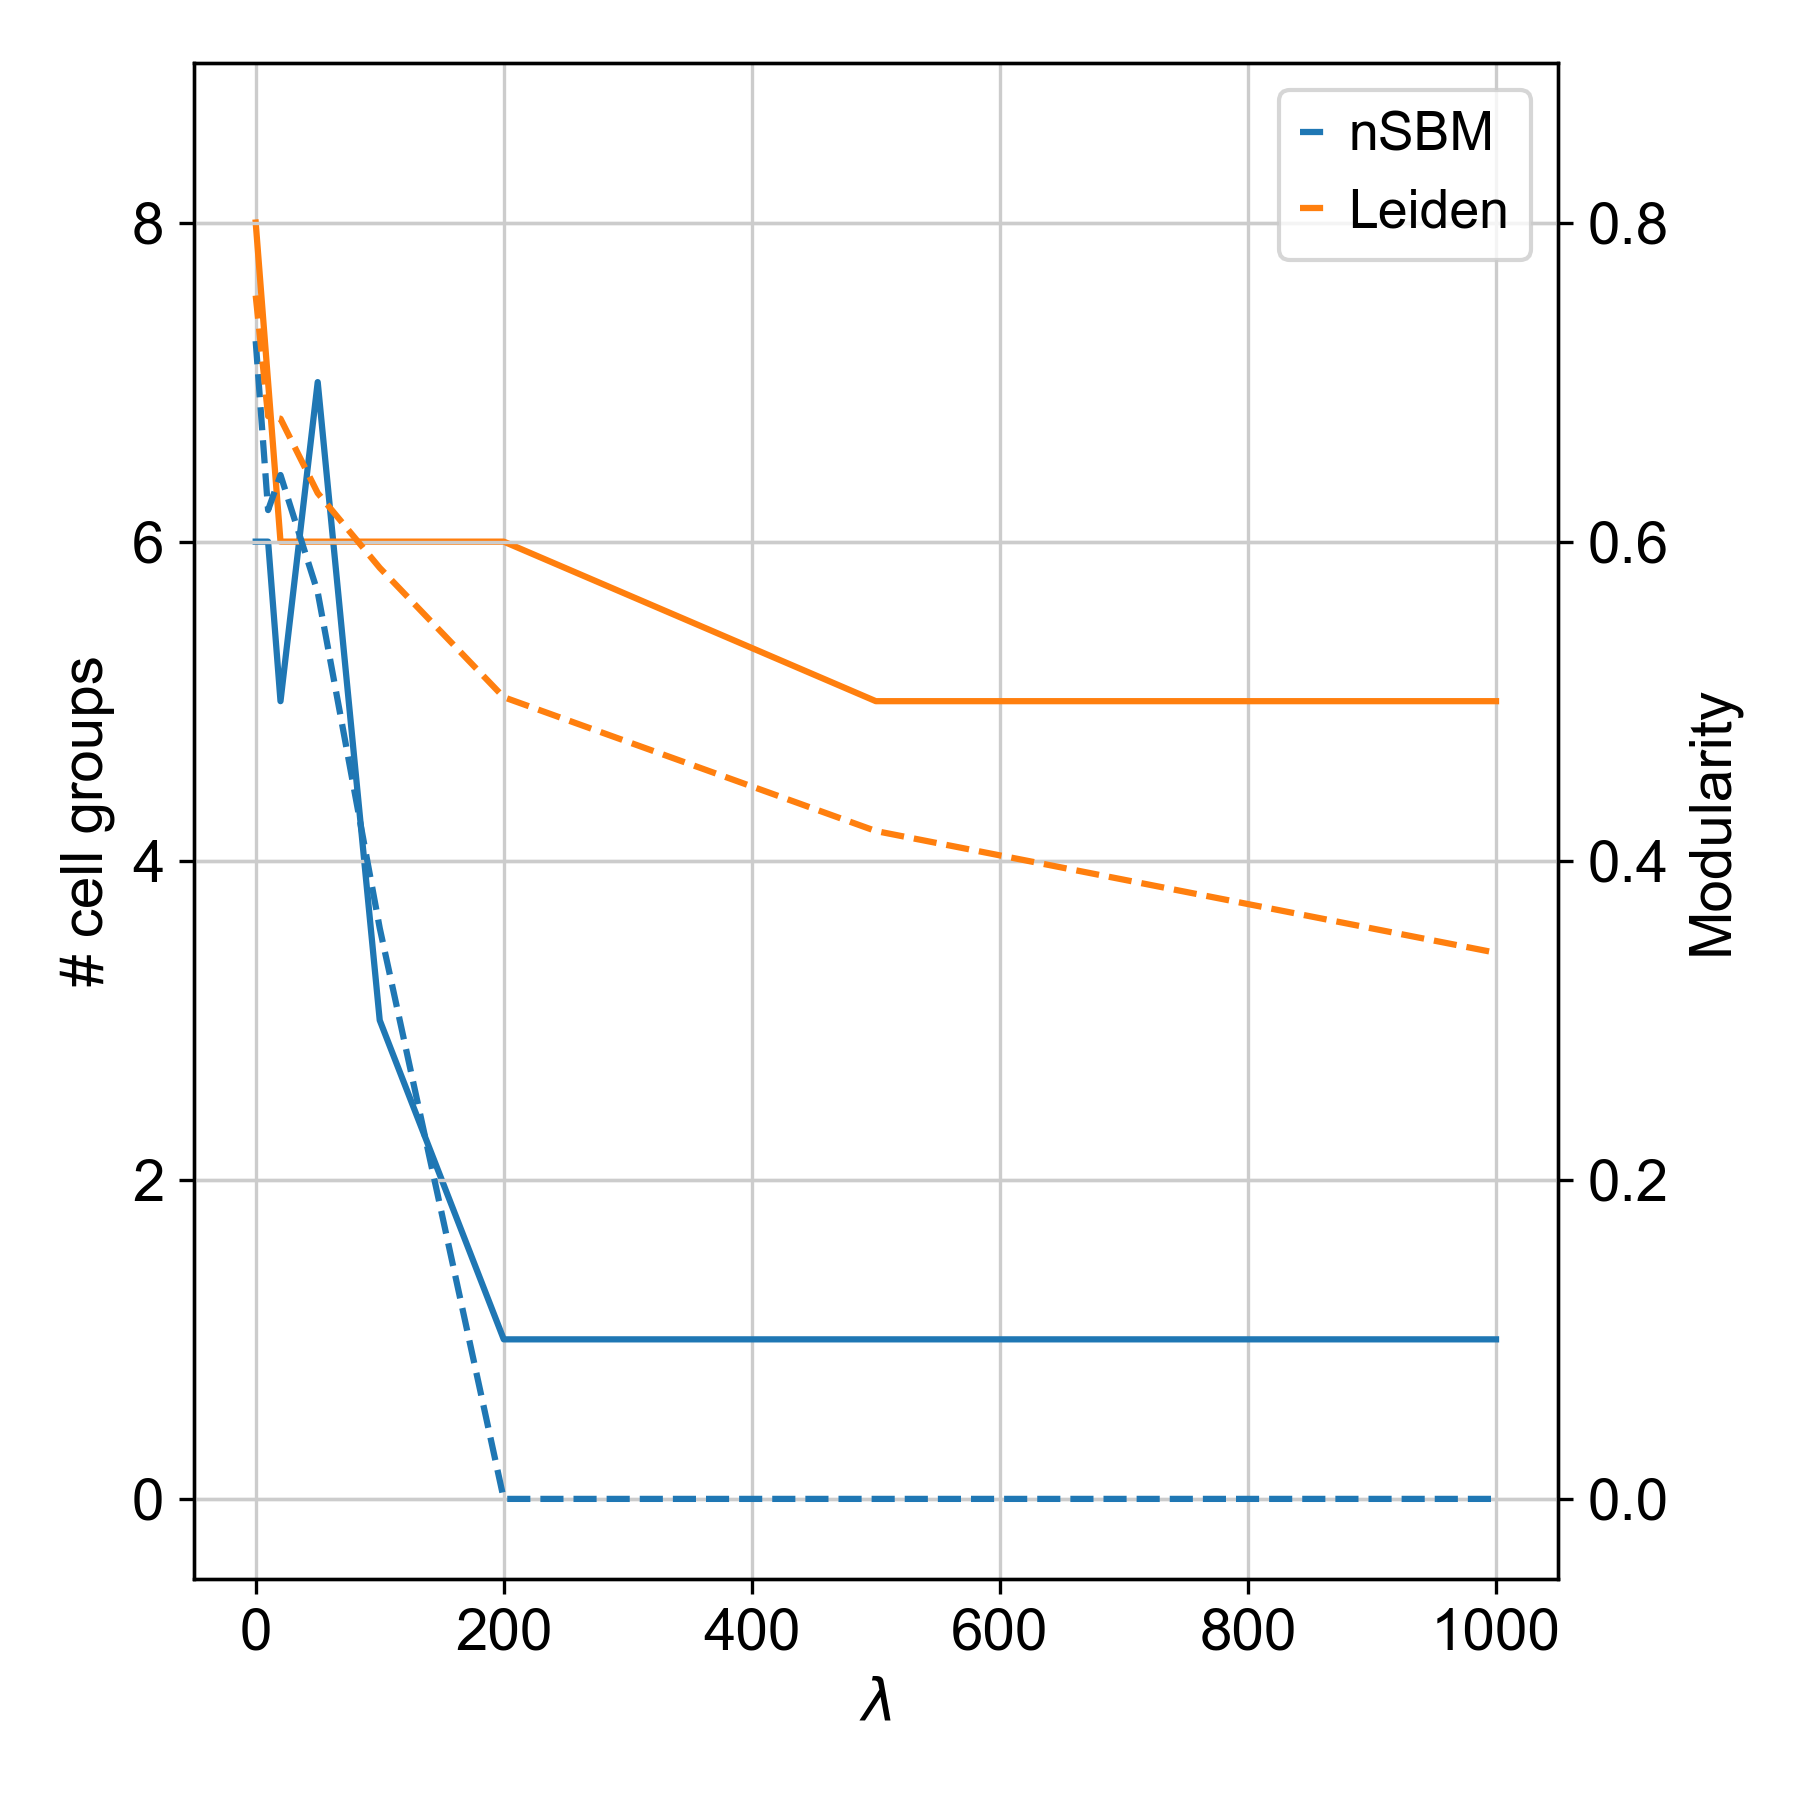
\includegraphics[keepaspectratio,width=\textwidth,height=0.6\textheight]{Tian_Random.png}
\caption[]{Identification of cell groups at different level of random noise. When random Poisson noise is added to the gene count martix, at increasing values of $\lambda$, a strategy based on optimization of modularity does return cell groups, whereas nSBM does not cluster cells when the noise exceeds a certain threshold (solid lines). The behaviour of the former approach follows the trend of the modularity (dashed lines), which is sustained at high levels independently from the level of noise.}\label{Figure_Random}
\end{figure}



\subsection*{Model hierarchy contains biological information}
The hierarchical model of cell groups implies that a relationship exists between groups. We next wanted to explore if the hierarchy proposed by the nSBM had a biological interpretation. To this end, we analysed data for hematopoietic differentiation \cite{paul_2015}, previously used to benchmark the consistency of cell grouping with differentiation trajectories by graph abstraction \cite{wolf_2019}. Standard processing of those data reveals three major branchings (Erythroids, Neutrophils and Monocytes) stemming from the progenitor cells (\nameref{S3_Fig}A). After applying nSBM, we identify 27 groups at level 3 of the hierarchy (\nameref{S3_Fig}B), compared to the 24 using Leiden method at default resolution (\nameref{S4_Fig}). We found that the hierarchy proposed by our model is consistent with the developmental model (Fig. \ref{Figure2}). Of note, we found that clustering with Leiden method produces cell groups that are mixed and split at different resolutions (0.1 - 1), in a non hierarchical manner (\nameref{S4_Fig}); we spotted several occurrences of such phenomenon, \emph{e.g.} group 9 at resolution $r=0.4$ splits into groups 0 and 6 at $r=0.3$ or group 3 at $r=0.6$ splits in groups 4, 8 and 12 at $r=0.5$.

In all, these data suggest that not only nSBM is able to identify consistent cell groups at different scales, but also that the hierarchy proposed by the model has a direct biological interpretation.

\begin{figure}[!h]
\centering
%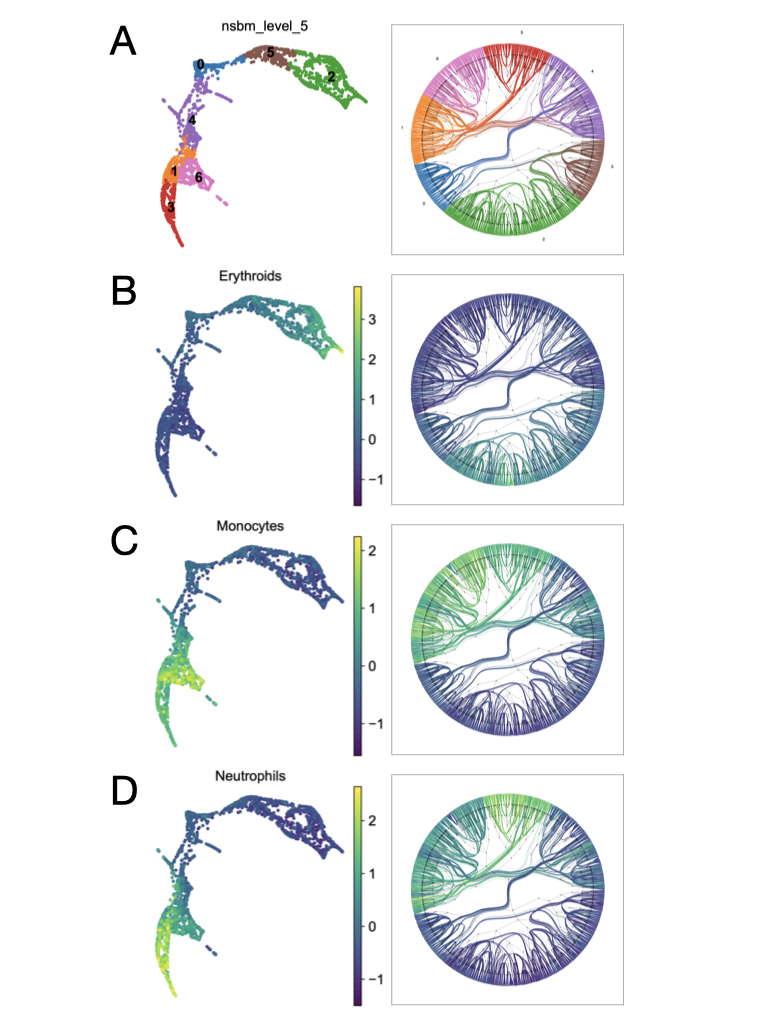
\includegraphics[keepaspectratio,width=\textwidth,height=0.55\textheight]{Figure_2.png}
\caption[]{Analysis of hematopoietic differentiation. Each panel presents a low dimensional embedding of single cells next to a radial tree representation of the nSBM hierarchy. Cells are colored according to groupings at level 5 of the hierarchy, group 0 marks the progenitor population (A). In subsequent panels, cells are colored using a signature of erythroid lineage (B), monocytes (C) or neutrophils (D).}\label{Figure2}
\end{figure}

\subsection*{Cell affinities can be used to evaluate cluster purity}
The computational framework underlying \emph{schist} calculates the model entropy, that is the amount of information required to describe a block configuration. Given that minimisation of such quantity can be used to perform model selection, it can be also used to evaluate the impact of modifying the assignment of a cell to a cluster. Once a model is minimised, \emph{schist} performs an exhaustive exploration of all model entropies resulting from moving all cells into all possible clusters. The differences in entropies could be interpreted as affinities of cells to given clusters. Such affinities are, in fact, probability values and could be used to evaluate the internal consistency of a given cell cluster. 

To this end we calculate the entropy of the group-wise distribution of cell affinities, which is maximal when all cells have affinity equal to 1 for a given group. We tested this idea on four datasets recently published to benchmark single cell technologies in the Human Cell Atlas project \cite{mereu_2020}; in particular, we chose two technologies resulting in high quality data: Quartz-seq2 \cite{sasagawa_2018} and Chromium 10x v3 \cite{zheng_2017}, and two technologies resulting in more noisy data: MARS-seq \cite{jaitin_2014} and iCell8 \cite{goldstein_2017} (Fig. \ref{Figure3}).

Cluster consistency is not a measure of the data quality, in fact we identify low consistency groups in all datasets. High consistency, instead, appears to be linked to the biological purity of the cells and it is inverse to the diversity index, estimated using cell annotation from the original paper. Consequently, filtering low consistency groups increases concordance with biological groups, at the cost of a reduced number of cells ( \nameref{S5_Fig}). 

Similarly, we can use cell affinities to derive a stability parameter, a measure of the tendency for a cell to be stably associated to given clusters at all levels of the hierarchy. To this end, we first calculate the cell-wise entropy $H_{i,h}$ of cell affinity at each hierarchy level \emph{h}, then we define the stability as $S_i = 1 - \max(H_i)$. While we conceived this measure to identify and exclude cells with dubious assignment, we found that it may be more useful to assess the general data quality: the fraction of cells having $S>0.95$ was 0.783, 0.795, 0.831 and 0.855 for the iCELL8, MARS-seq, Chromium 10x and Quartz-seq2 technology respectively, in line with the evaluation on increasing performances of those platforms in \cite{mereu_2020}.

\begin{figure}[!h]
\centering
%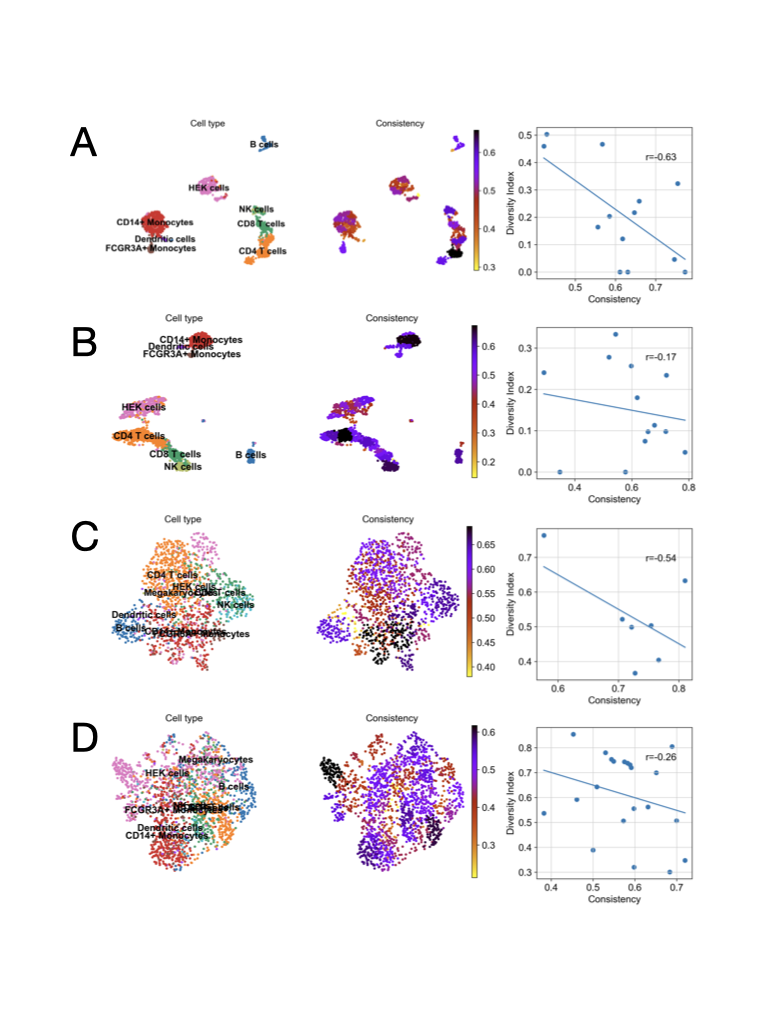
\includegraphics[keepaspectratio,width=\textwidth,height=0.6\textheight]{Figure_3.png}
\caption[]{Analysis of cell cluster consistency. Every panel reports a UMAP embedding of a PBMC + HEK293 cells profiled on different platform. Cells are annotated by cell type and by consistency value, which is assigned to cell clusters at nSBM level 1. The charts next to UMAPs show the correlation between consistency and diversity index for each cell cluster. Technologies showed here are (A) Chromium 10x v3, (B) Quartz-seq 2, (C) MARS-seq and (D) iCELL8.}\label{Figure3}
\end{figure}



%\subsection*{Hierarchic model constrains differential gene tests}
%Current approaches to test for gene markers in scRNA-seq data rely on pairwise or one-vs-rest comparisons among cell groups. This strategy assumes that cell groups are independent which, in general, may not be true. A notable exception is the recently introduced treeclimbR \cite{huang_2020} which has been specifically developed to perform differential tests over a tree structure. We reasoned that we could superpose the hierarchical structure inferred by \emph{schist} by fitting a linear model with mixed-effect, so that we model the dependencies using the inferred tree.


\subsection*{Analysis of runtimes}
Minimisation of the nSBM is a process that may require a large amount of computational resources. The analysis of a relatively small scRNA-seq dataset, such as the ones in \cite{mereu_2020}, may require several minutes to be processed. This could be a serious limitation to the adoption of nSBM in the analysis of single cell data, especially because several parameters should be tested. To overcome this limitation, it was suggested to let a greedy merge-split MCMC algoritthm \cite{peixoto_2020} to explore the solutions and stop iterations when the difference in entropy is below a defined threshold. We tested this approach on a commodity hardware (MacBook Air, dual core 1.6 GHz i5 processor, 16 GB RAM) and compared to the default approach. Results are reported in Table \ref{Table1}. The merge-split algorithm greatly reduces the time needed to propose the final model. In addition, the partitions found are largely overlapping the ones found by the default approach. 

\begin{table}[h!]
\centering
 \begin{tabular}{|| l c c c c  ||}
%  \begin{tabular}{|| m{7em} | m{5em} | m{7em} | m{7em} | m{5em} ||}
 \hline
 \textbf{Dataset} & \textbf{Cells} & \textbf{Minimize} & \textbf{Merge-split MCMC} & \textbf{Overlap} \\ [0.5ex] 
 \hline\hline
 sc-mixology \cite{tian_2019} & 860 & 01:11 & 00:03 & 0.884 \\ 
 \hline
 Quartzseq \cite{mereu_2020} & 1266 & 00:31 & 00:02 & 0.726 \\ 
 \hline
 MARS-seq \cite{mereu_2020} & 1401 & 00:29 & 00:08 & 0.834 \\
 \hline
 Chromium 10X \cite{mereu_2020} & 1523 & 00:40 & 00:04 & 0.695 \\
 \hline
 iCELL8 \cite{mereu_2020} & 1830 & 00:54 & 00:07 & 0.623 \\
 \hline
 Paul15 \cite{paul_2015} & 2730 & 02:37 & 00:10 & 0.575 \\ 
 \hline
 Planaria \cite{plass_2018} & 21612 & 13:12 & 03:29 & 0.589 \\
 \hline
% 4 & 545 & 18744 & 7560 \\
% \hline
% 5 & 88 & 788 & 6344 \\ [1ex] 
% \hline
\end{tabular}
\caption{Time required to minimise the nSBM using the default minimization method compared to the greedy merge-split MCMC. Times are expressed in mm:ss. Partition overlap measures concordance between the two models over the full hierarchy. Timing is the average after 3 initialisations.}
\label{Table1}
\end{table}


\section*{Conclusion}

Identification of cells sharing similar properties in single cell experiments is of paramount importance. A large number of approaches have been described, although the standardisation of analysis pipelines converged to methods that are based on modularity optimisation. We tackled the biological problem using a different approach, nSBM, which has several advantages over existing techniques. The most important advantage is the hierarchical definition of cell groups which eliminates the choice of an arbitrary threshold on clustering resolution. In addition, we showed that the hierarchy itself could have a biological interpretation, implying that the hierarchical model is a valid representation of the cell ensemble. Our approach introduces the evaluation of cluster consistency, which can be used to isolate cells with heterogeneous identity. Lastly, a statistical way to evaluate models is made available, allowing for reliable model selection. This last capability has the obvious advantage that the choice of parameters, hence the definition of cell clusters, could be conditioned to an evaluation metric which is robust and easy to understand (\emph{i.e.} the model entropy).

The major drawback of adopting this strategy is the substantial increase of runtimes. According to the developers of \emph{graph-tool}, runtimes are proportional to the number of edges in the neighbourhood graph and while it supports CPU-level parallelisation, a model minimisation is hundreds times slower than the extremely fast Leiden approach. Nevertheless, we show that a greedy merge-split MCMC algorithm can overcome this limitation, achieving performances that allow the usage of \emph{schist} on standard desktop hardware to analyse various single cell datasets.


\section*{Supporting information}

% Include only the SI item label in the paragraph heading. Use the \nameref{label} command to cite SI items in the text.
\paragraph*{S1 Fig.}
\label{S1_Fig}
{\bf Degree distribution of \emph{k}NN graphs.} Degree distribution of multiple \emph{k}NN graphs derived from scRNA-seq mixology datasets using variable number of Principal Components or number of neighbors. Each histogram shows the number of nodes (on y axis) within a specific degree bin (on x axis). Both the parameters influence the sparseness of the graph.

\paragraph*{S2 Fig.}
\label{S2_Fig}
{\bf nSBM performance after MCMC.}  Adjusted Rand Index for different \emph{k}NN graphs after MCMC run. Maximal ARI over all hierarchy level is shown. Darker color indicates higher concordance with the ground truth.

\paragraph*{S3 Fig.}
\label{S3_Fig}
{\bf Analysis of hematopoietic differentiation. }  (A) Low dimensional embedding of single cells colored by original cell type and pseudotime. (B) Cells are colored according to the nSBM grouping at level 3 of the hierarchy, next to a radial tree representation of the same model.

\paragraph*{S4 Fig.}
\label{S4_Fig}
{\bf Non hierarchical clustering at different resolution.}  Low dimension embedding of single cells for hematopoietic differentiation colored according to Leiden clustering at decreasing resolution, from 1.0 to 0.1. Lowering the distribution does not grant that cells are grouped in a hierarchical way, \emph{e.g.\ }group 3 at resolution \emph{r}=0.3 splits in groups 2 and 0 at resolution \emph{r}=0.2.

\paragraph*{S5 Fig.}
\label{S5_Fig}
{\bf Cluster consistency and cell type identification.} Adjusted Rand Index between cell clusters and cell type annotation filtering data at different cutoffs of consistency. Dot size is proportional to the number of cells remaining after filtering.

\section*{Acknowledgments}
We would like to thank Tiago de Paula Peixoto (Central European University, ISI Foundation) and Giovanni Petri (ISI Foundation) for the discussions and the precious hints. We also would like to thank all people at COSR, in particular Giovanni Tonon and Paolo Provero.

\nolinenumbers

% Either type in your references using
% \begin{thebibliography}{}
% \bibitem{}
% Text
% \end{thebibliography}
%
% or
%
% Compile your BiBTeX database using our plos2015.bst
% style file and paste the contents of your .bbl file
% here. See http://journals.plos.org/plosone/s/latex for 
% step-by-step instructions.
% 
\begin{thebibliography}{10}

\bibitem{svensson_2018}
Svensson V, Vento-Tormo R, Teichmann SA.
\newblock Exponential scaling of single-cell {RNA}-seq in the past decade.
\newblock Nature Protocols. 2018;13(4):599--604.
\newblock doi:{10.1038/nprot.2017.149}.

\bibitem{guo_2018}
Guo J, Grow EJ, Mlcochova H, Maher GJ, Lindskog C, Nie X, et~al.
\newblock The adult human testis transcriptional cell atlas.
\newblock Cell Research. 2018;28(12):1141--1157.
\newblock doi:{10.1038/s41422-018-0099-2}.

\bibitem{ventotormo_2018}
Vento-Tormo R, Efremova M, Botting RA, Turco MY, Vento-Tormo M, Meyer KB,
  et~al.
\newblock Single-cell reconstruction of the early maternal-fetal interface in
  humans.
\newblock Nature. 2018;563(7731):347--353.
\newblock doi:{10.1038/s41586-018-0698-6}.

\bibitem{rozenblattrosen_2020}
Rozenblatt-Rosen O, Regev A, Oberdoerffer P, Nawy T, Hupalowska A, Rood JE,
  et~al.
\newblock The Human Tumor Atlas Network: Charting Tumor Transitions across
  Space and Time at Single-Cell Resolution.
\newblock Cell. 2020;181(2):236--249.
\newblock doi:{10.1016/j.cell.2020.03.053}.

\bibitem{tirosh_2016}
Tirosh I, Izar B, Prakadan SM, Wadsworth MH, Treacy D, Trombetta JJ, et~al.
\newblock Dissecting the multicellular ecosystem of metastatic melanoma by
  single-cell {RNA}-seq.
\newblock Science. 2016;352(6282):189--196.
\newblock doi:{10.1126/science.aad0501}.

\bibitem{patel_2014}
Patel AP, Tirosh I, Trombetta JJ, Shalek AK, Gillespie SM, Wakimoto H, et~al.
\newblock Single-cell {RNA}-seq highlights intratumoral heterogeneity in
  primary glioblastoma.
\newblock Science. 2014;344(6190):1396--1401.
\newblock doi:{10.1126/science.1254257}.

\bibitem{neftel_2019}
Neftel C, Laffy J, Filbin MG, Hara T, Shore ME, Rahme GJ, et~al.
\newblock An integrative model of cellular states, plasticity, and genetics for
  glioblastoma.
\newblock Cell. 2019;178(4):835--849.e21.
\newblock doi:{10.1016/j.cell.2019.06.024}.

\bibitem{rosenberg_2018}
Rosenberg AB, Roco CM, Muscat RA, Kuchina A, Sample P, Yao Z, et~al.
\newblock Single-cell profiling of the developing mouse brain and spinal cord
  with split-pool barcoding.
\newblock Science. 2018;360(6385):176--182.
\newblock doi:{10.1126/science.aam8999}.

\bibitem{wagner_2018}
Wagner DE, Weinreb C, Collins ZM, Briggs JA, Megason SG, Klein AM.
\newblock Single-cell mapping of gene expression landscapes and lineage in the
  zebrafish embryo.
\newblock Science. 2018;360(6392):981--987.
\newblock doi:{10.1126/science.aar4362}.

\bibitem{plass_2018}
Plass M, Solana J, Wolf FA, Ayoub S, Misios A, Glažar P, et~al.
\newblock Cell type atlas and lineage tree of a whole complex animal by
  single-cell transcriptomics.
\newblock Science. 2018;360(6391).
\newblock doi:{10.1126/science.aaq1723}.

\bibitem{regev_2017}
Regev A, Teichmann SA, Lander ES, Amit I, Benoist C, Birney E, et~al.
\newblock The human cell atlas.
\newblock eLife. 2017;6.
\newblock doi:{10.7554/{eLife}.27041}.

\bibitem{wang_2017}
Wang B, Zhu J, Pierson E, Ramazzotti D, Batzoglou S.
\newblock Visualization and analysis of single-cell {RNA}-seq data by
  kernel-based similarity learning.
\newblock Nature Methods. 2017;14(4):414--416.
\newblock doi:{10.1038/nmeth.4207}.

\bibitem{lin_2017}
Lin P, Troup M, Ho JWK.
\newblock {CIDR}: Ultrafast and accurate clustering through imputation for
  single-cell {RNA}-seq data.
\newblock Genome Biology. 2017;18(1):59.
\newblock doi:{10.1186/s13059-017-1188-0}.

\bibitem{huh_2020}
Huh R, Yang Y, Jiang Y, Shen Y, Li Y.
\newblock {SAME}-clustering: Single-cell Aggregated Clustering via Mixture
  Model Ensemble.
\newblock Nucleic Acids Research. 2020;48(1):86--95.
\newblock doi:{10.1093/nar/gkz959}.

\bibitem{kiselev_2017}
Kiselev VY, Kirschner K, Schaub MT, Andrews T, Yiu A, Chandra T, et~al.
\newblock {SC3}: consensus clustering of single-cell {RNA}-seq data.
\newblock Nature Methods. 2017;14(5):483--486.
\newblock doi:{10.1038/nmeth.4236}.

\bibitem{li_2020}
Li X, Wang K, Lyu Y, Pan H, Zhang J, Stambolian D, et~al.
\newblock Deep learning enables accurate clustering with batch effect removal
  in single-cell {RNA}-seq analysis.
\newblock Nature Communications. 2020;11(1):2338.
\newblock doi:{10.1038/s41467-020-15851-3}.

\bibitem{krzak_2019}
Krzak M, Raykov Y, Boukouvalas A, Cutillo L, Angelini C.
\newblock Benchmark and Parameter Sensitivity Analysis of Single-Cell {RNA}
  Sequencing Clustering Methods.
\newblock Frontiers in genetics. 2019;10:1253.
\newblock doi:{10.3389/fgene.2019.01253}.

\bibitem{kiselev_2019}
Kiselev VY, Andrews TS, Hemberg M.
\newblock Challenges in unsupervised clustering of single-cell {RNA}-seq data.
\newblock Nature Reviews Genetics. 2019;20(5):273--282.
\newblock doi:{10.1038/s41576-018-0088-9}.

\bibitem{du_2018}
{Duò} A, Robinson MD, Soneson C.
\newblock A systematic performance evaluation of clustering methods for
  single-cell {RNA}-seq data.
\newblock F1000Research. 2018;7:1141.
\newblock doi:{10.12688/f1000research.15666.2}.

\bibitem{butler_2018}
Butler A, Hoffman P, Smibert P, Papalexi E, Satija R.
\newblock Integrating single-cell transcriptomic data across different
  conditions, technologies, and species.
\newblock Nature Biotechnology. 2018;36(5):411--420.
\newblock doi:{10.1038/nbt.4096}.

\bibitem{wolf_2018}
Wolf FA, Angerer P, Theis FJ.
\newblock {SCANPY}: large-scale single-cell gene expression data analysis.
\newblock Genome Biology. 2018;19(1):15.
\newblock doi:{10.1186/s13059-017-1382-0}.

\bibitem{blondel_2008}
Blondel VD, Guillaume JL, Lambiotte R, Lefebvre E.
\newblock Fast unfolding of communities in large networks.
\newblock Journal of Statistical Mechanics: Theory and Experiment.
  2008;2008(10):P10008.
\newblock doi:{10.1088/1742-5468/2008/10/P10008}.

\bibitem{traag_2019}
Traag VA, Waltman L, van Eck NJ.
\newblock From Louvain to Leiden: guaranteeing well-connected communities.
\newblock Scientific Reports. 2019;9(1):5233.
\newblock doi:{10.1038/s41598-019-41695-z}.

\bibitem{levine_2015}
Levine JH, Simonds EF, Bendall SC, Davis KL, Amir EaD, Tadmor MD, et~al.
\newblock Data-Driven Phenotypic Dissection of {AML} Reveals Progenitor-like
  Cells that Correlate with Prognosis.
\newblock Cell. 2015;162(1):184--197.
\newblock doi:{10.1016/j.cell.2015.05.047}.

\bibitem{newman_2004}
Newman MEJ, Girvan M.
\newblock Finding and evaluating community structure in networks.
\newblock Physical Review E, Statistical, Nonlinear, and Soft Matter Physics.
  2004;69(2 Pt 2):026113.
\newblock doi:{10.1103/{PhysRevE}.69.026113}.

\bibitem{traag_2011}
Traag VA, Van~Dooren P, Nesterov Y.
\newblock Narrow scope for resolution-limit-free community detection.
\newblock Physical Review E. 2011;84(1).
\newblock doi:{10.1103/{PhysRevE}.84.016114}.

\bibitem{reichardt_2006}
Reichardt J, Bornholdt S.
\newblock Statistical mechanics of community detection.
\newblock Physical Review E. 2006;74(1).
\newblock doi:{10.1103/{PhysRevE}.74.016110}.

\bibitem{lhnemann_2020}
{Lähnemann} D, {Köster} J, Szczurek E, {McCarthy} DJ, Hicks SC, Robinson MD,
  et~al.
\newblock Eleven grand challenges in single-cell data science.
\newblock Genome Biology. 2020;21(1):31.
\newblock doi:{10.1186/s13059-020-1926-6}.

\bibitem{fortunato_2007}
Fortunato S, {Barthélemy} M.
\newblock Resolution limit in community detection.
\newblock Proceedings of the National Academy of Sciences of the United States
  of America. 2007;104(1):36--41.
\newblock doi:{10.1073/pnas.0605965104}.

\bibitem{guimer_2004}
{Guimerà} R, Sales-Pardo M, Amaral LAN.
\newblock Modularity from fluctuations in random graphs and complex networks.
\newblock Physical Review E. 2004;70(2).
\newblock doi:{10.1103/{PhysRevE}.70.025101}.

\bibitem{baran_2019}
Baran Y, Bercovich A, Sebe-Pedros A, Lubling Y, Giladi A, Chomsky E, et~al.
\newblock {MetaCell}: analysis of single-cell {RNA}-seq data using K-nn graph
  partitions.
\newblock Genome Biology. 2019;20(1):206.
\newblock doi:{10.1186/s13059-019-1812-2}.

\bibitem{xu_2015}
Xu C, Su Z.
\newblock Identification of cell types from single-cell transcriptomes using a
  novel clustering method.
\newblock Bioinformatics. 2015;31(12):1974--1980.
\newblock doi:{10.1093/bioinformatics/btv088}.

\bibitem{miao_2020}
Miao Z, Moreno P, Huang N, Papatheodorou I, Brazma A, Teichmann SA.
\newblock Putative cell type discovery from single-cell gene expression data.
\newblock Nature Methods. 2020;17(6):621--628.
\newblock doi:{10.1038/s41592-020-0825-9}.

\bibitem{holland_1983}
Holland PW, Laskey KB, Leinhardt S.
\newblock Stochastic blockmodels: First steps.
\newblock Social networks. 1983;5(2):109--137.
\newblock doi:{10.1016/0378-8733(83)90021-7}.

\bibitem{peixoto_2017}
Peixoto TP.
\newblock Nonparametric Bayesian inference of the microcanonical stochastic
  block model.
\newblock Physical review E. 2017;95(1-1):012317.
\newblock doi:{10.1103/{PhysRevE}.95.012317}.

\bibitem{karrer_2011}
Karrer B, Newman MEJ.
\newblock Stochastic blockmodels and community structure in networks.
\newblock Physical Review E, Statistical, Nonlinear, and Soft Matter Physics.
  2011;83(1 Pt 2):016107.
\newblock doi:{10.1103/{PhysRevE}.83.016107}.

\bibitem{peixoto_2013}
Peixoto TP.
\newblock Parsimonious module inference in large networks.
\newblock Physical Review Letters. 2013;110(14):148701.
\newblock doi:{10.1103/{PhysRevLett}.110.148701}.

\bibitem{peixoto_2014}
Peixoto TP.
\newblock Efficient Monte Carlo and greedy heuristic for the inference of
  stochastic block models.
\newblock Physical Review E, Statistical, Nonlinear, and Soft Matter Physics.
  2014;89(1):012804.
\newblock doi:{10.1103/{PhysRevE}.89.012804}.

\bibitem{peixoto_2014_h}
Peixoto TP.
\newblock Hierarchical Block Structures and High-Resolution Model Selection in
  Large Networks.
\newblock Physical Review X. 2014;4(1):011047.
\newblock doi:{10.1103/{PhysRevX}.4.011047}.

\bibitem{tian_2019}
Tian L, Dong X, Freytag S, Lê~Cao KA, Su S, {JalalAbadi} A, et~al.
\newblock Benchmarking single cell {RNA}-sequencing analysis pipelines using
  mixture control experiments.
\newblock Nature Methods. 2019;16(6):479--487.
\newblock doi:{10.1038/s41592-019-0425-8}.

\bibitem{kang_2018}
Kang HM, Subramaniam M, Targ S, Nguyen M, Maliskova L, {McCarthy} E, et~al.
\newblock Multiplexed droplet single-cell {RNA}-sequencing using natural
  genetic variation.
\newblock Nature Biotechnology. 2018;36(1):89--94.
\newblock doi:{10.1038/nbt.4042}.

\bibitem{mereu_2020}
Mereu E, Lafzi A, Moutinho C, Ziegenhain C, {McCarthy} DJ, {Álvarez-Varela} A,
  et~al.
\newblock Benchmarking single-cell {RNA}-sequencing protocols for cell atlas
  projects.
\newblock Nature Biotechnology. 2020;38(6):747--755.
\newblock doi:{10.1038/s41587-020-0469-4}.

\bibitem{sasagawa_2018}
Sasagawa Y, Danno H, Takada H, Ebisawa M, Tanaka K, Hayashi T, et~al.
\newblock Quartz-Seq2: a high-throughput single-cell {RNA}-sequencing method
  that effectively uses limited sequence reads.
\newblock Genome Biology. 2018;19(1):29.
\newblock doi:{10.1186/s13059-018-1407-3}.

\bibitem{zheng_2017}
Zheng GXY, Terry JM, Belgrader P, Ryvkin P, Bent ZW, Wilson R, et~al.
\newblock Massively parallel digital transcriptional profiling of single cells.
\newblock Nature Communications. 2017;8:14049.
\newblock doi:{10.1038/ncomms14049}.

\bibitem{jaitin_2014}
Jaitin DA, Kenigsberg E, Keren-Shaul H, Elefant N, Paul F, Zaretsky I, et~al.
\newblock Massively parallel single-cell {RNA}-seq for marker-free
  decomposition of tissues into cell types.
\newblock Science. 2014;343(6172):776--779.
\newblock doi:{10.1126/science.1247651}.

\bibitem{goldstein_2017}
Goldstein LD, Chen YJJ, Dunne J, Mir A, Hubschle H, Guillory J, et~al.
\newblock Massively parallel nanowell-based single-cell gene expression
  profiling.
\newblock {BMC} Genomics. 2017;18(1):519.
\newblock doi:{10.1186/s12864-017-3893-1}.

\bibitem{paul_2015}
Paul F, Arkin Y, Giladi A, Jaitin DA, Kenigsberg E, Keren-Shaul H, et~al.
\newblock Transcriptional heterogeneity and lineage commitment in myeloid
  progenitors.
\newblock Cell. 2015;163(7):1663--1677.
\newblock doi:{10.1016/j.cell.2015.11.013}.

\bibitem{wolf_2019}
Wolf FA, Hamey FK, Plass M, Solana J, Dahlin JS, {Göttgens} B, et~al.
\newblock {PAGA}: graph abstraction reconciles clustering with trajectory
  inference through a topology preserving map of single cells.
\newblock Genome Biology. 2019;20(1):59.
\newblock doi:{10.1186/s13059-019-1663-x}.

\bibitem{peixoto_2020}
Peixoto TP.
\newblock Merge-split Markov chain Monte Carlo for community detection.
\newblock arXiv. 2020;doi:{arXiv:2003.07070}.

\end{thebibliography}



\end{document}

